% =====================================================================
% Promise Completeness, Not Model Capability
% arXiv submission source (cs.CY primary, cs.SE cross-list)
% v5 (2026-10-29): assertion lead-ins aligned with deadlines (A4/A7 "By
%                  mid-2027" -> "By end-2027"; A5 -> "By end-August 2027").
% v4 (2026-10-29): A2 win condition softened (task-composition breakdown as
%                  corroboration); A4 deadline -> 2027-12-31 with evidence-
%                  insufficient rule; A7 deadline -> 2027-12-31.
% v3 (2026-10-29): A5 deadline corrected to 2027-08-31 (Veracode publishes
%                  annually in July; the previous 2027-06-30 preceded the data).
% v2 (2026-10-28): Appendix A "Falsifiable Predictions (A1-A7)" added;
%                  no changes to Sections 1-8.
% Compile with pdflatex (recommended: Overleaf or arXiv online compilation).
% Figures must stay in ./figures/ next to this file:
%   acad_sanyinzi_en.png  acad_qibu_en.png  acad_jinzita_en.png  acad_jieduan_en.png
% =====================================================================
\documentclass[11pt]{article}

\usepackage[margin=2.5cm]{geometry}
\usepackage{graphicx}
\usepackage{amsmath}
\usepackage{booktabs}
\usepackage{array}
\usepackage[hidelinks]{hyperref}

\title{Promise Completeness, Not Model Capability: The Structural Ceiling
of Full Automation and the Cultivation of Human Evaluative Judgment}
\author{Lei Dai}
\date{October 2026}

\begin{document}
\maketitle

\begin{abstract}
Rapid progress in the capability of large language models has given rise to
two popular claims. The first: ``AI will catch up with humans''---given
continued scalable improvement, models will eventually replace humans in
complex tasks, including software development. The second: ``old knowledge
no longer needs to be learned''---since the old human ways of working will
be superseded anyway, the new generation can complete tasks directly with
AI, without acquiring the knowledge of the old mode of production. This
paper is a study of the societal impact of science and technology: it
subjects both claims to a systematic examination, investigating the social
boundaries of AI-driven automation expansion in production organization,
responsibility assignment, and talent-cultivation institutions. To this end
we propose the \emph{promise completeness} framework: whether a task can be
fully automated is not decided by how capable the model is, but by the
conjunction of three factors---definitional completeness of the task
specification, computational feasibility of verification or solution, and
social acceptability of assigning execution responsibility to machines. On
this framework the paper argues three propositions. \textbf{(P1)} The
boundary of full automation is structurally decoupled from model-capability
growth: AI will take over promise-complete subspaces, but will not become
the principal agent of complex production. \textbf{(P2)} In domains where
production knowledge and evaluative knowledge are coupled, human evaluative
judgment depends on ``pain memory''---learning from errors made with
one's own hands and bearing their consequences---which cannot be acquired
from observing AI-generated surface-level data; talent cultivation must
therefore preserve a four-stage path from handwriting the basics, through a
painful closed loop and predict-and-verify practice, to directing and
reviewing AI. \textbf{(P3)} Organizational responsibility capacity is an
independent hard constraint on automation expansion; it grows far more
slowly than model capability, so review and accountability roles will
remain the bottleneck for the foreseeable future. This paper reports no new
controlled experiments; it is a conceptual-analysis study built on published
empirical literature and historical cases.

\medskip
\noindent\textbf{Keywords:} AI-assisted development; automation boundary;
promise completeness; responsibility capacity; skill formation;
human-in-the-loop
\end{abstract}

\section{Introduction}
Over the past two years, two claims have circulated in public discussion of
AI and production relations. \textbf{Claim one: ``AI will catch up with
humans''}---as long as scalable capability improvement continues, AI will
be able to replace humans in a wide range of tasks, including highly
complex ones such as software development. \textbf{Claim two: ``old
knowledge no longer needs to be learned''}---since existing human workers
will eventually be displaced by AI, the next generation can simply use AI
to complete tasks and need not learn the knowledge of the old mode of
production.

One of these judgments concerns ``how far AI can go''; the other concerns
``how people still need to learn''. Together they determine how
individuals and organizations should invest over the next five to ten
years, and they jointly shape the evolution of labor-market structure,
responsibility institutions, and talent-cultivation systems---which is
exactly the object of study of this paper as research on the societal
impact of science and technology. Yet both claims lack an intermediate
link: what decides whether a task can be handed over to a machine
entirely? The default answer---``it is decided by model capability''---does
not match the empirical facts. For software tasks, compilation, unit
testing, and static checking are already essentially fully automated, while
operating-system kernels, distributed-consensus protocols, and
safety-critical systems are still required, even in the most optimistic
projections, to retain human review. For rule-complete board games, Go can
be played machine-against-machine, yet criminal sentencing in any
rule-of-law society is not permitted to be handed to a machine.

The thesis of this paper is: \textbf{whether a task can be fully automated
is decided by the conjunction of the three promise-completeness
factors---definitional completeness, computational feasibility, and social
acceptability---not by model capability.} Around this thesis the paper
makes three contributions:

(1) It proposes and formalizes the \textbf{three-factor promise-completeness
framework} (Section~3), gives a unified cross-domain decision procedure, and
analyzes its characteristic failure mode, ``apparent completeness.''
Unlike existing task-suitability frameworks (such as SML
\cite{sml_aea,sml_science}), which infer ``what machines can do now'' from
task characteristics, our framework takes responsibility assignment as an
independent factor and addresses the normative boundary of ``where, in
principle, there should be no place without a human'';

(2) It applies the framework to software production, giving a
\textbf{seven-step implementation framework for subspace-wise gradual
automation} with three deployment variants (Section~4), and analyzes
cross-subspace failure modes and governance responses using the Boeing 737
MAX accidents and the Rust project's LLM governance policy as cases;

(3) It argues for the \textbf{non-outsourcability of evaluative judgment}
(Section~5) and for \textbf{responsibility capacity as an independent hard
constraint} (Section~6), and derives from these the four-stage
talent-cultivation path.

This paper reports no new controlled experiments; all empirical evidence
comes from published research, surveys, and accident investigations.
Section~7 discusses the limitations of this choice explicitly.

\section{Related Work}
\subsection{Effectiveness Evidence for AI-Assisted Development and the
Perception--Measurement Gap}
Evidence on the effectiveness of AI coding tools is highly divergent. In
controlled experiments, laboratory tasks with GitHub Copilot reported a
55--56\% speedup \cite{copilot}; an enterprise-grade randomized controlled
trial (RCT) at Google measured a speedup of roughly 21--26\%
\cite{google_rct}; whereas the RCT published by METR in July 2025---sixteen
senior open-source developers completing 246 real tasks on mature
repositories they had maintained for an average of more than five
years---measured that using early-2025 AI tools made them \emph{19\%
slower}, while the developers expected a 24\% speedup beforehand and still
perceived a 20\% speedup afterwards \cite{metr}. It should be noted that in
METR's February 2026 update, returning participants measured an 18\%
speedup and newly recruited participants a 4\% slowdown, both with
confidence intervals crossing zero; the original estimate was declared a
historical snapshot of a specific tool and setting \cite{metr}. An industry
study by DX covering 121,000 developers shows a different side: 92.6\% of
developers use AI coding assistants every month and self-report saving
about four hours per week, but organization-level productivity gains have
entered a plateau of roughly 10\%, while AI-generated code has risen to
26.9\% of production code \cite{dx}.

These results do not contradict one another; together they point to the
core evidence type used in this paper: the \textbf{perception--measurement
gap}. Self-reported efficiency and objective throughput can diverge for
long periods (in METR the two differed by nearly 40 percentage points
\cite{metr}); any automation inference based on ``developers feel faster''
therefore requires independent verification. Effectiveness also depends
strongly on the task environment and on participants' familiarity with the
context---in greenfield codebases and in mature critical systems, the sign
of the same tool can flip \cite{metr,google_rct}.

\subsection{Levels of Automation and Human Factors}
The human--computer-interaction literature has long provided models of
levels of automation: Parasuraman et al.\ characterized automation along
four stages (information acquisition, analysis, decision selection, action
implementation) with ten levels \cite{parasuraman2000}, and the automotive
engineering community popularized the SAE J3016 levels 0--5. Parasuraman
and Riley systematically summarized use, misuse, disuse, and abuse of
automation \cite{parasuraman1997}; among their findings,
``automation bias''---the human tendency to over-trust machine
output---remains one of the most robust human-factor findings in
human-in-the-loop systems. The Boeing 737 MAX accidents (in which failures
of MCAS, an ``automated subspace,'' propagated through interfaces into the
flight crew's handling space) are a canonical case of automation bias
compounded by responsibility mismatch \cite{boeing}. The three-factor and
seven-step frameworks of this paper can be read as a refinement and
operationalization of this levels-of-automation tradition along the
dimension of responsibility assignment.

\subsection{Responsibility Assignment: The Responsibility Gap and Moral
Crumple Zones}
Matthias introduced the ``responsibility gap'': the behavior of learning
machines cannot, on the causal chain, be traced back to an accountable
human \cite{matthias}. Elish describes the ``moral crumple zone,'' in
which human operators of automated systems are positioned as responsibility
``absorbers''---nominally responsible, but in substance lacking the
judgment and the information that the responsibility presupposes
\cite{elish}. A July 2026 position paper from Berkeley RDI, \emph{Towards
Autonomous Software Development}, proposed a 0--III classification of
autonomy levels for software development (analogous to driving-automation
levels) and pointed to the transfer of responsibility in the course of
autonomization and to gaps in the legal framework of software
responsibility \cite{berkeleyrdi}. This paper complements \cite{berkeleyrdi}:
theirs characterizes ``how responsibility is progressively transferred from
humans to machines''; ours answers ``which responsibilities will
structurally remain on the human side, and why,'' and further connects the
responsibilities that remain with human talent-cultivation institutions.

\subsection{Empirical Evidence on Skill Formation}
In January 2026 Anthropic published an RCT in which 52 mostly junior
engineers learned the unfamiliar Trio asynchronous library: the AI group
scored 17 percentage points lower on a subsequent test (50\% versus 67\%,
nearly two letter grades), with the largest gap on debugging questions;
task-time differences were not significant \cite{anthropic_rct}. The key
moderating variable is \emph{mode of use}: participants who delegated code
generation to AI entirely scored below 40\%, while participants who used AI
to ask conceptual questions and wrote code with their own hands scored
above 65\% \cite{anthropic_rct}. A meta-analysis by Alanazi of 35 controlled
studies (2020--2024) gives the isomorphic picture: AI assistance
significantly improves performance scores on programming tasks (SMD $=$
0.86, 95\% CI $[0.36, 1.37]$) but has almost no effect on learning outcomes
or self-assessed understanding (SMD $= 0.16$, 95\% CI $[-0.23, 0.55]$,
nonsignificant) \cite{alanazi}. Section~5 of this paper reads this body of
evidence as empirical support for the claim that evaluative knowledge
cannot be learned from surface-level performance data.

\subsection{The Task-Characteristics Tradition of Occupational Automation
Assessment}
Judging ``what can be automated'' at the occupation and task level has a
long tradition. Frey and Osborne estimated the probability of
computerization for occupations using three engineering bottlenecks---perception
and manipulation, creative intelligence, and social intelligence
\cite{freyosborne}; their insight was that ``structural constraints exist
beyond capability,'' but the bottlenecks remain capability-side
heuristics. The Suitability for Machine Learning (SML) framework of
Brynjolfsson et al.\ judges the ML suitability of a task by its
characteristics---whether the objective function is clear, whether training
data are available, whether feedback is timely, and so on
\cite{sml_aea,sml_science}; it is the conceptual ancestor of our C and F
factors. Shao et al., addressing the era of AI agents, propose a task-level
auditing framework and the Human Agency Scale (H1--H5), which sorts tasks
into four zones---automation green light, red light, R\&D opportunity, and
low priority---by ``practitioner willingness $\times$ expert capability
assessment,'' explicitly framing their scale as a human-side complement to
the SAE ``AI-first'' view \cite{shao}.

Our relationship to this lineage is inheritance plus divergence. We inherit
its task-level (rather than occupation-level) unit of analysis. We diverge
in three ways. First, we extend specification completeness from ``having an
objective and data'' to \emph{promise completeness} that covers hidden
corners such as boundary conditions and systemic risks, and we characterize
its failure mode as ``apparent completeness.'' Second, we establish social
acceptability and responsibility assignment as an independent factor (A)
\emph{on a par with} definitional completeness and computational
feasibility, connecting to the responsibility-gap \cite{matthias} and moral
crumple zone \cite{elish} literatures. Third, SML and HAS answer the
``positive'' question (what can be done now, what people want now), while
our three factors answer the ``normative'' question---where, in principle
and in institution, there cannot be a place without a human. The three are
complementary: the positive distribution moves fast with tool iteration,
while normative constraints decide the direction and the endpoint of the
movement.

\section{Promise Completeness: The Boundary of Full Automation Is Decided
by Three Factors}
\subsection{Framework Definition}
\textbf{Definition (promise completeness).} A task $T$ is promise-complete
if and only if all three of the following factors hold:

\textbf{C (definitional completeness):} the acceptance criteria of $T$ can
be made explicit to a sufficiently fine granularity---not only the happy
path, but also boundary conditions, exception handling, performance
constraints, and systemic risks, i.e., all the ``unsaid corners''---and the
specification can be kept continuously aligned with the delivered artifact;

\textbf{F (computational feasibility):} there exists a process executable
at acceptable cost that gives a sufficiently strong decision or solution
for the correctness of candidate outputs against the specification;

\textbf{A (social acceptability):} social institutions (law, ethics,
industry practice) are willing to assign the execution responsibility of
the task to a machine, and to accept the machine as the bearer of
responsibility, or its output as the basis of responsibility, when errors
occur.

\textbf{Proposition (structural boundary).} A task $T$ can be fully
automated $\Longleftrightarrow$ $C(T) \wedge F(T) \wedge A(T)$. The three
factors are in \emph{conjunction}: if any one fails, ``human-in-the-loop''
is not a transitional form caused by technological immaturity, but a
structural component of that task (Figure~\ref{fig:factors}).

\begin{figure}[t]
\centering
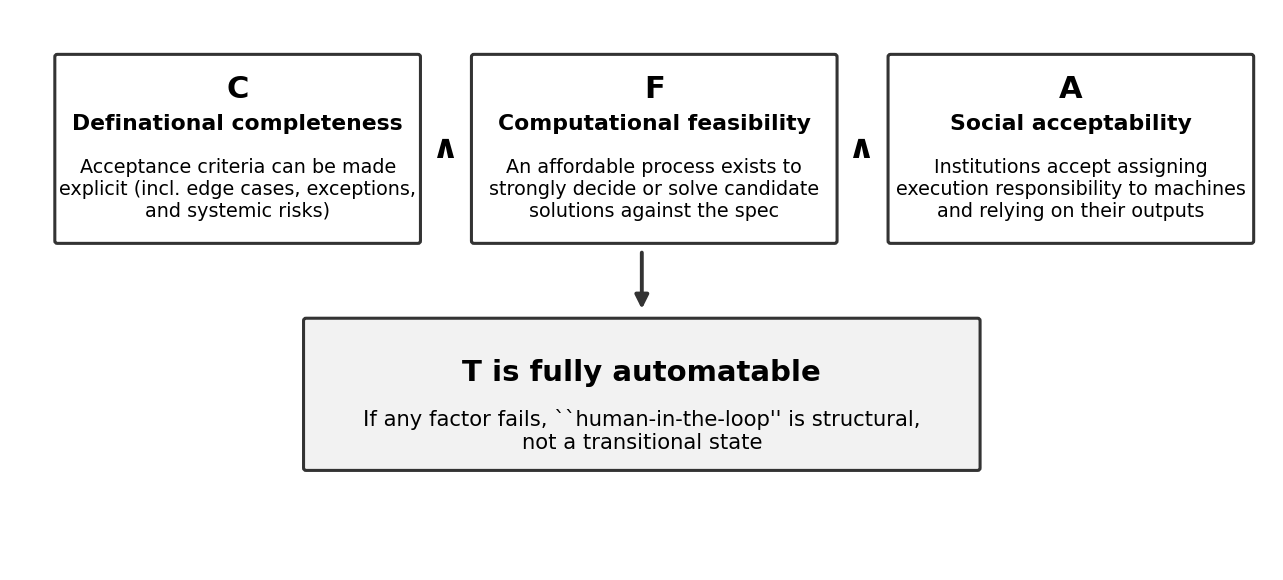
\includegraphics[width=0.95\linewidth]{figures/acad_sanyinzi_en.png}
\caption{The three promise-completeness factors and their conjunction.}
\label{fig:factors}
\end{figure}

We deliberately do not list ``model capability'' as a factor. Model
capability decides ``how far machines can help humans \emph{inside} a
promise-incomplete space''; promise completeness decides ``whether such a
space can, in principle, have no place for a human.'' The former improves
rapidly with scale; the latter is decided by task semantics and
institutional structure. The two are decoupled---this is the precise
statement of P1.

\subsection{Cross-Domain Evidence}
``Promise completeness'' is \textbf{a term introduced by this paper} (as of
October 2026, a literature search found no prior academic use); it separates
``whether a task's promise is complete enough to be entrusted to a
machine'' from the vague ``whether capability is enough.'' Its difference
from task-suitability concepts such as SML
\cite{sml_aea,sml_science} is that suitability measures how friendly a task
is to current technology, whereas promise completeness measures whether the
task specification itself can be closed to the degree of ``no missing
clause even with no human in the loop.''

Table~\ref{tab:domains} organizes representative domains by the three
factors. Domains with all three values present serve to test the
discriminating power of the framework: for software tasks, low-level tasks
are high on all three factors and have been essentially automated, whereas
high-level tasks are low on all three and must remain human-led---this is
precisely why the public debate on ``whether AI-written code is reliable''
remains unresolved: the two sides are talking about different subspaces.

\begin{table}[t]
\centering
\small
\setlength{\tabcolsep}{3.5pt}
\begin{tabular}{p{4.0cm}p{2.6cm}p{2.2cm}p{2.9cm}p{3.0cm}}
\toprule
\textbf{Domain / task} & \textbf{C: definitional} &
\textbf{F: computational} & \textbf{A: social} &
\textbf{Automation outcome} \\
\midrule
Textiles, machine tools, bookkeeping & High (metrics formalizable) &
High & High & Full machine takeover \\
Go (the game) & High (complete rules) & High (search $+$ learning) &
High (no responsibility assignment) & AlphaGo-style full takeover
\cite{alphago} \\
Protein structure prediction & High (energy-minimizing conformation) &
Low (exact solving unaffordable) & High & AI opened the space of
approximate solutions \cite{alphafold} \\
Capital / serious-crime sentencing & Medium (rules codifiable) & Medium &
$\approx$0 (society insists on human judgment) & Machines cannot be the
deciding subject \\
Software, low level (compilation, unit tests, lint) & High & High & High &
Already highly automated \\
Software, high level (OS kernels, distributed consensus, safety-critical) &
Low (many hidden corners) & Low & Low & Human-led, AI-assisted \\
\bottomrule
\end{tabular}
\caption{Cross-domain instantiations of the three-factor framework.}
\label{tab:domains}
\end{table}

\subsection{Failure Mode: Apparent Completeness}
The most dangerous failure is not a factor being explicitly false, but
\textbf{apparent completeness}---a promise that is complete on paper while
materially missing key clauses. Credit derivatives before the 2008
financial crisis are the canonical example: contract terms were precise,
pricing models elegant, and the promise of any single contract highly
complete; but the clause ``systemic risk'' was missing from the promise of
the system as a whole, and the absence was statistically insignificant and
invisible in normal times, until the crisis cashed it in \cite{fcic}. The
``passes the tests'' status of AI-generated code is structurally
isomorphic: test coverage is finite, and clauses not written into
tests---maintainability, architectural fit, long-term evolvability---become
visible only later. The implication for automation is: \textbf{however high
F and A are, the truth of C can only be maintained through continuous
supervision}---this sets up the monitoring obligation of Section~4 and the
responsibility-capacity argument of Section~6.

\section{Subspace-Wise Gradual Automation: A Seven-Step Framework}
\subsection{The Partitioning Principle}
The natural corollary of the three factors is: do not ask ``can the whole
system be automated?'' but ``\emph{whose} promise, in which subspace, is
complete?'' The best teacher is the aircraft autopilot: the same system
allocates primacy by the promise completeness of each flight
phase---automatic in cruise, human-led in takeoff and landing, and manual
takeover mandatory at the decision height on approach. It should be noted
that phasing human--machine roles is a mature tradition---SAE J3016 and the
Parasuraman model \cite{parasuraman2000} represent the ``AI-first'' view,
and the Human Agency Scale \cite{shao} gives the human-side H1--H5 view;
our partitioning criterion differs from all three: \textbf{it is based
neither on machine capability nor on human willingness, but on the promise
completeness of the subspace}---complete, and it is handed over;
incomplete, and it stays on the human side; and whatever is handed over can
be taken back at any time the completeness assumption fails. We import this
principle into software production: \textbf{decompose the system into
subspaces, judge the three factors for each subspace independently,
allocate human--machine primacy by completeness, and carry a monitoring
obligation for the continued validity of each completeness assumption.}

\subsection{The Seven-Step Framework}
Figure~\ref{fig:seven} gives the complete flow of the seven-step framework;
its textual principle is a single sentence: \textbf{before AI acts, the
completeness of that subspace's promise must be proved; after AI acts, the
continued validity of that completeness assumption must be monitored.}

\begin{figure}[t]
\centering
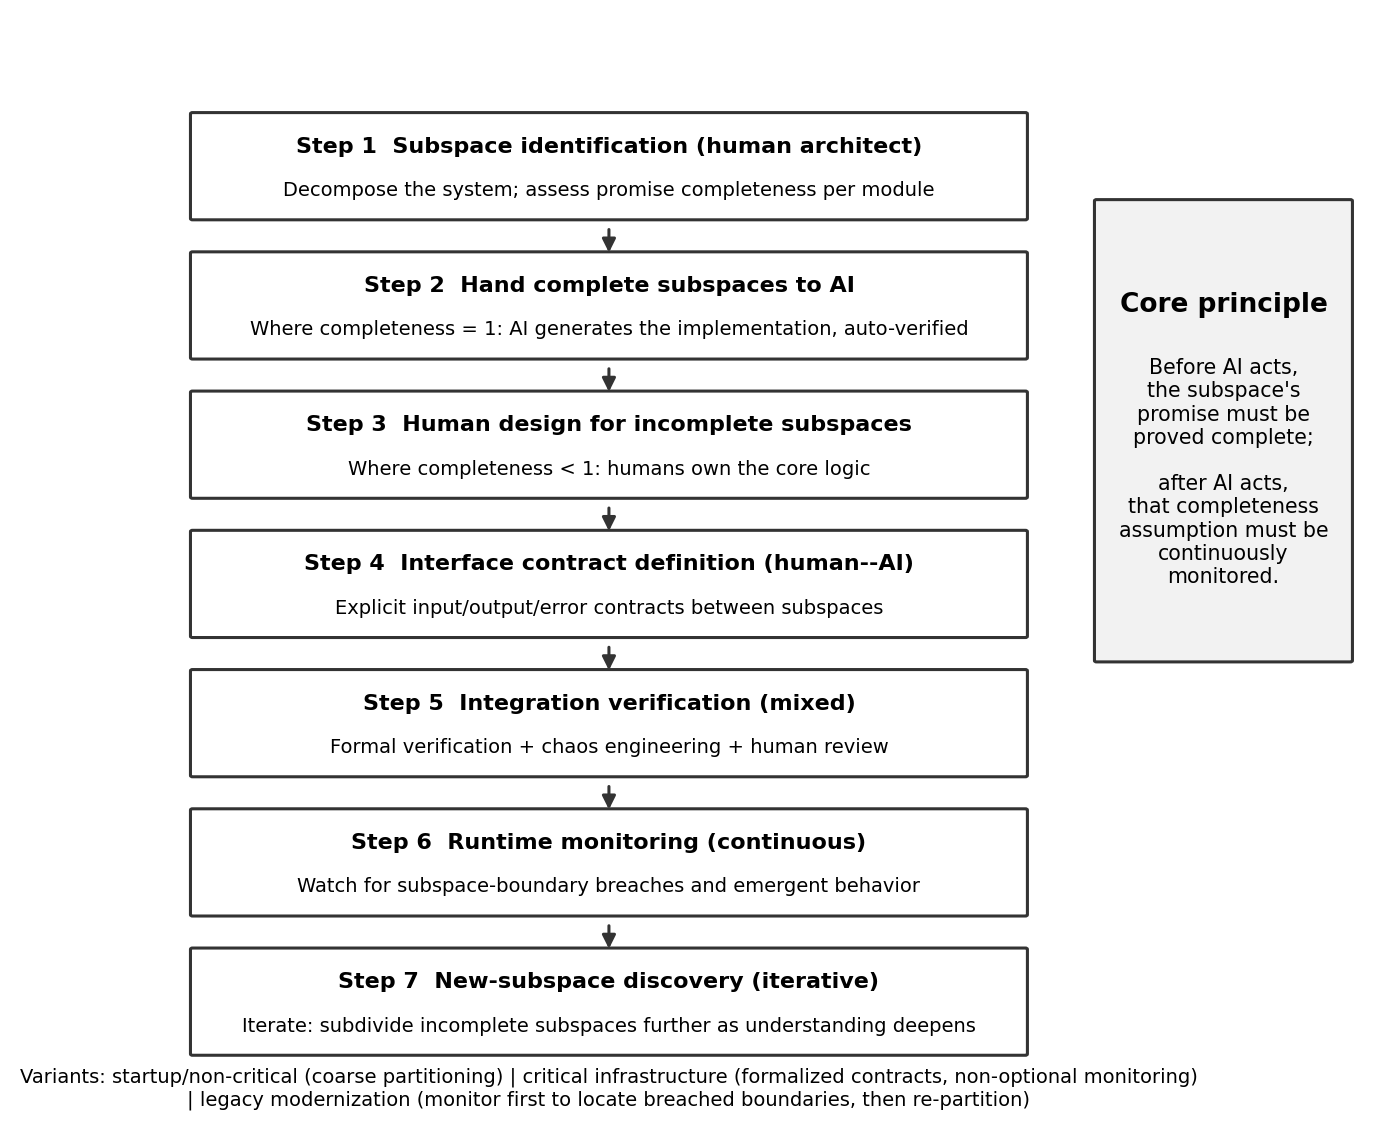
\includegraphics[width=0.8\linewidth]{figures/acad_qibu_en.png}
\caption{The seven-step implementation framework and its three deployment
variants.}
\label{fig:seven}
\end{figure}

\subsection{Three Deployment Variants}
The same framework is tailored to three organizational contexts:
\textbf{(1) startups / non-critical systems}---perform a coarse-grained
subspace partitioning first, automate only the ``obviously complete''
parts, and keep interface contracts and monitoring lightweight;
\textbf{(2) critical infrastructure}---completeness assessments are
strict, interface contracts must be formalized, and runtime monitoring is
non-optional; \textbf{(3) legacy modernization}---run monitoring first to
locate where historical evolution has breached subspace boundaries, then
re-partition gradually following Step~7.

\subsection{Failure Modes and Governance Responses}
The most dangerous failure of subspace automation is not a fault inside a
subspace, but \textbf{a failure crossing subspace boundaries}: on the Boeing
737 MAX, a fault of MCAS, an ``automated subspace,'' propagated through
interfaces into the ``human subspace,'' while the flight crew did not know
of that subspace's existence and in substance lost the ability to take over
\cite{boeing}. In general, cross-subspace failures come in three types:
\textbf{fuzzy boundaries} (humans do not know what the machine is
managing), \textbf{state asynchrony} (when the machine disengages, the
human receives incomplete context), and \textbf{switching latency} (the
takeover decision lags the time constant of the failure).

The open-source community has produced an isomorphic governance response.
In August 2026 the Rust project adopted a formal LLM policy for
rust-lang/rust: LLMs may be used for answering, analysis, review, and
translation, but \textbf{must not implement on one's behalf}; LLM review
conclusions may not replace human review; concealing usage is treated as a
Code-of-Conduct violation; and a circuit-breaker mechanism pauses
acceptance when LLM-created merge PRs exceed half of the total within any
six-week period \cite{rustblog,rustpolicy}. In substance, this policy
treats ``which subspaces AI is allowed to dominate'' as a governance object
that requires explicit delimitation and continuous measurement---the same
direction as our framework.

\section{Why Evaluative Judgment Cannot Be Outsourced}
\subsection{The Two Decoupling Questions and Pseudo-Decoupling}
To judge whether an industry can be taken over wholesale, one needs to ask
only two questions: \textbf{knowledge decoupling}---can someone who cannot
produce nevertheless evaluate the outcome effectively? And \textbf{process
decoupling}---once production has started, can it run to completion without
a human watching? Textiles, machine tools, and bookkeeping answer ``yes''
to both, so machines took over wholesale; artistic creation, strategic
decision-making, complex medical care, and legal adjudication answer ``no''
to both---\textbf{evaluation is part of production}, and humans must stay
in the loop. High-level software development belongs to the latter group:
evaluating a piece of code requires understanding its semantics, and the
act of coding is itself pervaded by micro-evaluations (naming,
abstraction, trade-offs).

What demands more vigilance is \textbf{pseudo-decoupling}: much automation
does not genuinely satisfy the two questions; it quietly redefines
``good'' instead (Table~\ref{tab:pseudo}).

\begin{table}[t]
\centering
\small
\begin{tabular}{p{3.4cm}p{4.6cm}p{6.2cm}}
\toprule
\textbf{Original task} & \textbf{Reduced automated version} &
\textbf{Quietly discarded dimensions} \\
\midrule
Weave a good piece of cloth & Strength $\geq$ 50\,N, color fastness
$\geq$ grade 4 & Hand feel, breathability, texture over time \\
Cook a good meal & One standard burger in 3 minutes & Flavor depth,
cultural context, emotional connection \\
Write good software & Code that passes the tests & Maintainability,
architectural fit, long-term evolvability \\
\bottomrule
\end{tabular}
\caption{Pseudo-decoupling: automation's quiet redefinition of ``good.''}
\label{tab:pseudo}
\end{table}

The test question for pseudo-decoupling is: \textbf{is what was simplified
away precisely the most valuable part?}

\subsection{Pain Memory and the Three-Tier Pyramid}
In the production of complex products, production knowledge and evaluative
knowledge are \textbf{coupled}: cultivating the ability to evaluate product
quality cannot avoid hands-on participation in production. The root reason
is that genuine judgment comes from \textbf{``pain memory''---errors made
with one's own hands and paid for with real consequences}; failure modes
only sediment into intuition that precedes deliberation in the next
decision when they are bound to real costs (rework, accidents,
accountability). We divide evaluative capability into three tiers
(Figure~\ref{fig:pyramid}): a1 rule memory (verbalizable, teachable by
curriculum), a2 pattern memory (demonstrable, transmissible by
apprenticeship), and a3 intuitive memory (grows only from hands-on
practice). \textbf{The higher the tier, the less one can bypass hands-on
practice}; observing AI-generated outcomes stays at the surface level and
cannot substitute for acquiring the base tiers.

\begin{figure}[t]
\centering
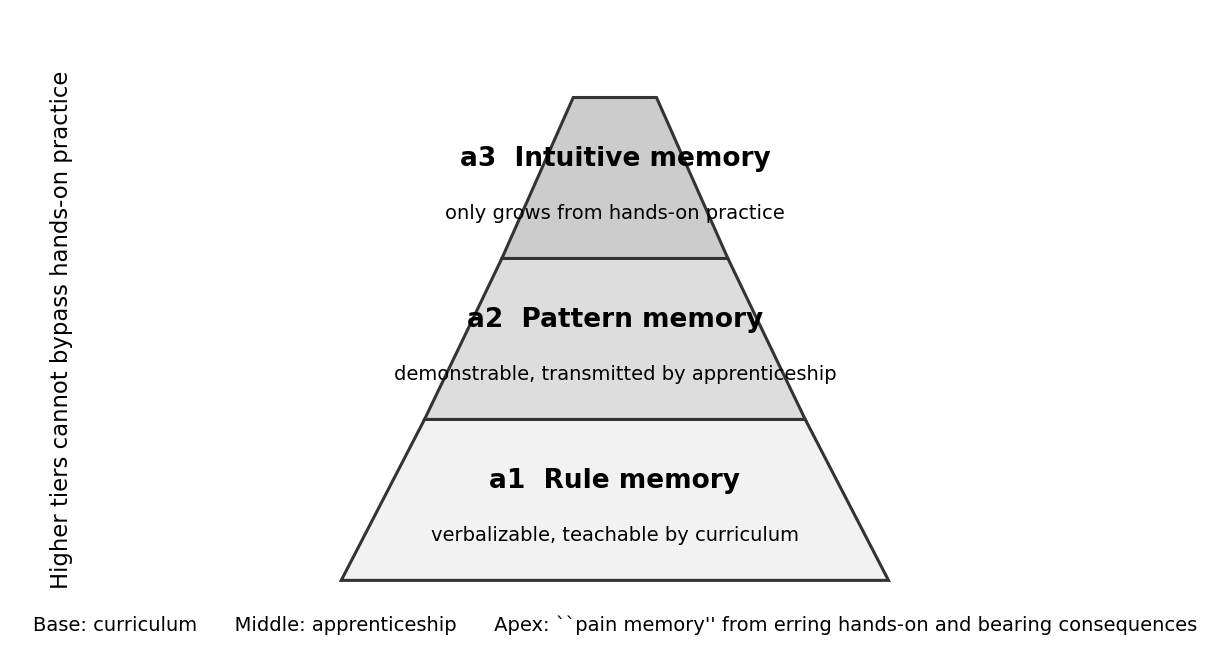
\includegraphics[width=0.75\linewidth]{figures/acad_jinzita_en.png}
\caption{The three-tier pyramid of evaluative capability: higher tiers
depend more on hands-on practice.}
\label{fig:pyramid}
\end{figure}

Software engineering harbors an underrated fact: software has no physical
embodiment, and its execution can only be simulated in the mind
\emph{---hand-writing code is the only mandatory deductive training in
which ``it simply does not run unless you get it right.''} The closed loop
of the senior engineer---writing with one's own hands (forced to reason
precisely about variable states and control flow), maintaining it oneself
(getting burned by mines planted by one's own code three years earlier),
bearing the consequences (failures, data corruption), forming intuition
(``where it will hurt'' appearing before thought)---every step is a
component of pain memory.

\subsection{Empirical Evidence}
Three bodies of evidence support the mechanism. First, Anthropic's RCT
shows that learners who delegated code generation to AI scored 17
percentage points lower on the test, with the largest gap on debugging,
while learners who used AI to learn concepts and wrote code with their own
hands were unaffected \cite{anthropic_rct}---\textbf{what decides gain or
loss is not whether AI is used, but whether the hands-on link is skipped}.
Second, the meta-analysis of 35 studies shows significant improvement in
task performance but no significant improvement in conceptual
understanding \cite{alanazi}---``finishing'' and ``learning'' can be
statistically separated, which is exactly the projection of the knowledge
decoupling assumption into learning settings. Third, the error profile of
AI is systematically different from that of humans: human errors are mostly
predictable patterns (fatigue typos, logical slips), whereas AI errors
often ``look right'' semantically; Veracode's continuous scanning of more
than 100 models found that 45\% of generated code contains OWASP Top-10
vulnerabilities, and newer, larger models were not safer \cite{veracode}---
\textbf{without hand-writing fundamentals, one cannot even see the errors}.

\subsection{The Four-Stage Cultivation Path}
The normative claim of this paper is not ``reject AI,'' but
\textbf{the order cannot be scrambled}: the first two stages deliberately
forgo AI, and the last two stages learn to orchestrate it
(Figure~\ref{fig:stages}).

\begin{figure}[t]
\centering
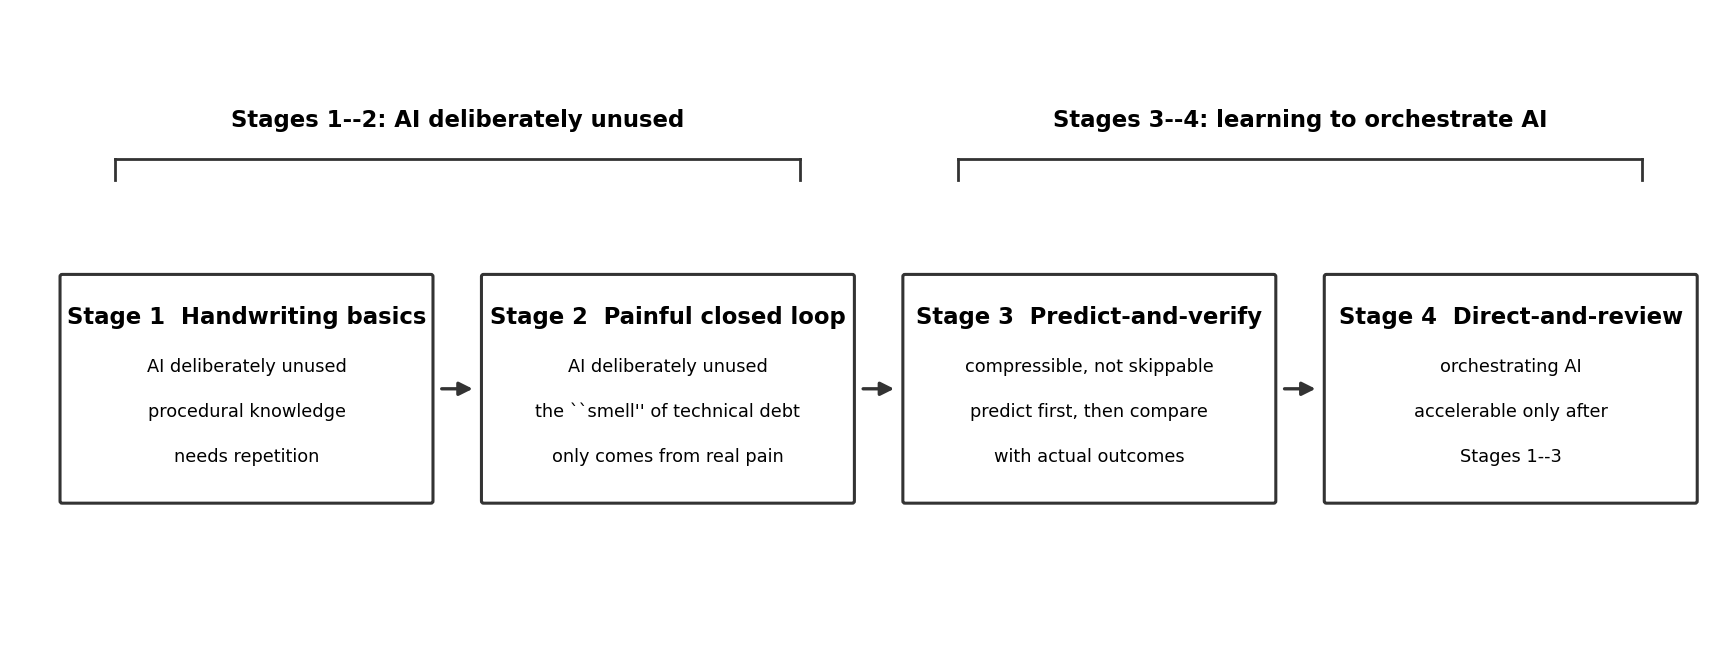
\includegraphics[width=0.98\linewidth]{figures/acad_jieduan_en.png}
\caption{The four-stage cultivation path.}
\label{fig:stages}
\end{figure}

Stage~1 ``handwriting the basics'': procedural knowledge needs sufficient
repetition to be internalized. Stage~2 ``painful closed loop'': the
``smell'' of technical debt can only come from real pain and cannot be
simulated. Stage~3 ``predict-and-verify'': compressible in part, but not
skippable. Stage~4 ``direct-and-review'': accelerable, \textbf{provided
Stages 1--3 are complete}.

A horizontal institutional comparison deserves note. Medicine requires
years of residency plus licensure plus individual accident liability;
aviation, despite autopilots, still requires pilots to fly manually on a
regular basis and to pass simulator checks; law prohibits practice without
apprenticeship. Software engineering is only decades old as a discipline:
no license, no residency, extremely high societal tolerance---it should
demand stricter institutions, yet in reality it is looser. It must be
honestly pointed out that almost no institution in industry currently
cultivates talent along this path: corporate KPIs generally push AI usage
rates up, and ``not using AI'' can even become a reason for a poor
performance review. This path is, for now, more ``normative'' than
``positive''---\textbf{but precisely because nobody does it, whoever walks
it first will possess judgment that others cannot replace}.

\section{Responsibility Capacity: A Hard Constraint Beyond Model Capability}
\subsection{The Layering of Responsibility}
Twisting the first two threads together: even if models keep improving,
there remains a hard constraint that does not depend on model
capability---\textbf{how much responsibility human organizations can carry}.
Berkeley RDI calls this the ``responsibility transfer'' problem in the
course of autonomization \cite{berkeleyrdi}; the corresponding concepts in
the literature are the responsibility gap \cite{matthias} and the moral
crumple zone \cite{elish}: human reviewers are positioned as responsibility
``absorbers''---their signature lands in the approval box, while in
substance they lack the judgment and the information that the
responsibility presupposes.

Responsibility can be divided into three layers: \textbf{L1 operational
responsibility} (code review, test verification)---partially outsourcable
to AI, but what is outsourced is execution, not responsibility itself;
\textbf{L2 judgment responsibility} (architectural trade-offs, risk
assessment)---hard to outsource, because it demands accountability for the
hidden corners not written into the specification, exactly where factor C
is weakest; \textbf{L3 strategic and ethical responsibility} (value
judgments, interest coordination, accountability)---until AI obtains the
qualification of a ``responsibility-bearing subject,'' it can only be
carried by humans.

\subsection{Three Bodies of Data Converging}
Three public datasets point to the same constraint from different sides.
Black Duck's 2026 survey of software developers: 52\% of respondents
consider manual review the primary bottleneck of AI-generated code, and
51\% consider security testing a bottleneck; in teams where AI-written code
grew by more than 50\%, 57\% regard security testing and vulnerability
repair as the biggest bottleneck \cite{blackduck}. METR's RCT showed senior
developers getting slower with AI on mature repositories, with
self-assessment and actual outcome pointing in opposite directions
\cite{metr}. Veracode's continuous scanning shows 45\% of AI-generated code
containing security vulnerabilities, with no improvement across model
generations \cite{veracode}. McKinsey's comparative analysis provides the
positive corroboration: the companies benefiting significantly are not
those that ``shipped a tool,'' but those that restructured the development
process and turned people into orchestrators of AI \cite{mckinsey}---the
bottleneck is not on the generation side, but on the review and
responsibility-acceptance side.

\subsection{Corollaries}
\textbf{Responsibility capacity is relatively rigid in the short run and can
be slowly expanded in the long run by institutional innovation} (clearer
responsibility law, more effective review toolchains, specialized review
divisions of labor), \textbf{but its rate of expansion is far slower than
the growth rate of AI capability} (compare the generation-over-generation
stagnation in \cite{veracode} with the continued leaps in model
capability). Therefore review, judgment, and accountability roles will long
remain the bottleneck; the stronger the model, the more qualified review
each unit of output requires, and the more ``responsibility capacity''
becomes the true constraint on automation expansion---this is the content
of P3.

\section{Discussion and Limitations}
\textbf{Relation to existing position papers.} This paper shares with the
Berkeley RDI autonomy-level taxonomy \cite{berkeleyrdi} the view that
responsibility is redistributed as autonomization proceeds; the difference
is that our three-factor framework supplies a decision criterion for
``which subspaces cannot or should not become fully autonomous in
principle,'' and explicitly connects the responsibilities that remain on
the human side to talent-cultivation institutions (Section~5) and to the
organizational bottleneck (Section~6).

\textbf{Falsifiability.} The three-factor framework issues a testable
verdict for every concrete domain: if a domain judged ``not fully
automatable'' by the framework is stably and fully automated in practice
(in the sense of no human review and the machine bearing responsibility),
the framework needs revision. The framework also allows failures of
``apparent completeness'' to be identified ex post (as in \cite{fcic}).

\textbf{Inherent limits of conceptual analysis.} This paper reports no new
controlled experiments; the frameworks of Sections~3 and~4 are induced from
historical cases and public research, carrying the risk of single-case
inference; the factor-value judgments involve unavoidable subjectivity, and
the ``medium'' and ``low'' entries in Table~\ref{tab:domains} should be
read as hypotheses awaiting testing rather than measurements.

\textbf{Indirectness of the mechanistic evidence.} The direct evidence for
``pain memory'' currently comes from behavioral and learning science
(\cite{anthropic_rct,alanazi}) and from indirect support in the skill
acquisition literature; a direct neuroscientific characterization is still
missing. Research on trust similarly shows that trust in humans and trust
in AI are separable constructs, and only the former exhibits stable neural
correlates \cite{trust}---consistent with the argument direction of ``AI
lacks a shared biological basis,'' but corroboration rather than proof.

\textbf{Timeliness.} Empirical conclusions in this field have short
half-lives: METR's original estimate was partially revised by its own
update within eight months \cite{metr}, and all tool-capability data cited
here represent only their publication dates. The framework-level
propositions (P1--P3) are designed to be insensitive to tool iteration, but
the path recommendation of Section~5.4 needs recalibration as the
institutional environment changes.

\section{Conclusion}
Three sentences gather the paper. AI's \textbf{capability boundary} is
demarcated by promise completeness, not by model capability. The human
\textbf{value anchor} is evaluative judgment, and judgment can only be
cultivated with one's own hands---it cannot be learned from surface-level
data. The \textbf{ratio} between the two is constrained by responsibility
capacity: however strong the model becomes, it only makes the review list
longer. Accordingly, each of ``AI will catch up with humans'' and ``old
knowledge no longer needs to be learned'' is half right: AI will take over
more and more of the promise-complete subspaces---that much is fact; but
the further up one goes, the more evaluation, judgment, and accountability
return to humans, and there is no shortcut to that capability.

\appendix
\section{Falsifiable Predictions (A1--A7)}
\label{app:predictions}
Every claim in this paper can be cast as an assertion with an observable,
third-party-verifiable win/loss condition and a deadline. The seven
assertions below cover P1--P3 and the framework's failure modes; each
lists its baseline, deadline (with the anchoring rationale), and our
confidence. At each deadline the assertion receives a three-way verdict
(win / loss / evidence insufficient); the framework passes a round if at
least five assertions win with none lost, and the corresponding
propositions require revision if two or more are lost (the loss condition
of A6 is a weak one, and A4 may end \emph{evidence insufficient} if no
independent replication exists by its deadline; both are excluded from
this accounting).

\subsection*{A1. Human review remains mandatory in safety-critical domains
(P1) --- confidence 80\%}
\textbf{Assertion.} By mid-2027, flagship coding models still cannot
deliver fully automated, review-free production output in
promise-incomplete domains such as OS kernels, distributed consensus, or
safety-critical systems; human review remains mandatory in mainstream
certification standards (DO-178C, ISO 26262, Common Criteria).
\textbf{Win.} At the deadline, at least one mainstream safety-critical
certification standard still mandates human review, and no third-party
verified case of review-free delivery exists. \textbf{Loss.} At least one
third-party verified case of fully automated, review-free delivery in the
domains above. \textbf{Deadline.} 2027-06-30 (one full model generation;
if the mandatory-review status were to erode, public signals of standard
revision would appear within a year).

\subsection*{A2. Automation growth stays inside promise-complete
subspaces (P1) --- confidence 70\%}
\textbf{Assertion.} By end-2027, growth in the AI-generated share of code
remains concentrated in scaffolding, test boilerplate, and
compilation-verifiable low-level code; human primacy in high-level domains
is unchanged. \textbf{Win.} An industry survey of DX caliber (or equivalent) shows the
AI-generated share of code continuing to rise, and no formal ``AI-led''
engineering practice exists in high-level safety-critical domains (the
task-composition breakdown counts as corroboration, not a hard condition,
at whatever granularity the survey actually publishes). \textbf{Loss.} A widely adopted engineering practice in which AI
leads design and delivery in kernel/consensus/safety-critical domains.
\textbf{Deadline.} 2027-12-31 (covers the full data window of the 2027 DX
annual survey plus the minimal window for observing practice change).
\textbf{Baseline.} DX research: AI-generated code at 26.9\% of production
code (Nov 2025--Feb 2026 window) \cite{dx}.

\subsection*{A3. Generation-side growth does not convert into
organizational output (P3) --- confidence 65\%}
\textbf{Assertion.} By end-2027, the AI code share keeps rising while
organization-level productivity gains remain stalled at a $\leq$15\%
plateau (baseline: roughly 10\% in DX 2026), with the bottleneck still on
the review and responsibility-acceptance side. \textbf{Win.} At least one
authoritative industry survey replicates ``share up, output plateau,''
and manual review or security testing is still listed as the top
bottleneck by $\geq$50\% of teams (baseline: 52\%/51\% in Black Duck
2026). \textbf{Loss.} Organization-level productivity gains exceed 20\%
and are confirmed by at least two independent sources. \textbf{Deadline.}
2027-12-31 (captures the refresh of both the DX and Black Duck annual
surveys by year-end). \textbf{Baselines.} DX $\sim$10\% plateau
\cite{dx}; Black Duck, \emph{The State of AI-Powered Software
Development} (June 2026, $n=831$) \cite{blackduck}.

\subsection*{A4. The delegation learning deficit replicates (P2) ---
confidence 70\%}
\textbf{Assertion.} By end-2027, at least one independent controlled study
replicates the 2026 Anthropic RCT: learners who fully delegate code
generation score $\geq$10 percentage points lower on
comprehension/debugging tests than hands-on learners. \textbf{Win.} At
least one published, controlled study replicates the direction and
magnitude. \textbf{Loss.} At least two independent studies show no
significant negative effect of delegated use on learning outcomes. (If no
independent replication exists by the deadline, the verdict is
\emph{evidence insufficient} and A4 is excluded from the round's
accounting, as with A6.)
\textbf{Deadline.} 2027-12-31 (controlled studies have no fixed release
schedule; the deadline sits almost two years after the original RCT,
covering any reasonable research cycle).
\textbf{Baseline.} Shen \& Tamkin, arXiv:2601.20245: AI group 50\% versus
control 67\%, largest gap on debugging \cite{anthropic_rct}.

\subsection*{A5. AI vulnerability rates show no generational improvement
(P2) --- confidence 60\%}
\textbf{Assertion.} By end-August 2027, under the same measurement protocol the
next generation of flagship models still exhibits a vulnerability rate of
$\geq$30\%: ``bigger $\neq$ safer'' continues to hold. \textbf{Win.} The
Veracode protocol (OWASP Top-10 scanning, 100+ models) or an
equivalent-caliber report shows $\geq$30\% for the new generation.
\textbf{Loss.} The same-caliber report shows $<$20\%, or a recognized
benchmark demonstrates that new models are systematically safer than the
human average. \textbf{Deadline.} 2027-08-31 (Veracode publishes its
report annually in July; the deadline sits within one month after the
expected 2027 edition, spanning one full generation turnover).
\textbf{Baselines.} Veracode 2025 edition: 45\% of generated code contains
OWASP Top-10 vulnerabilities; 2026 edition: 56\% pass rate, officially
``virtually unchanged'' \cite{veracode}.

\subsection*{A6. An apparent-completeness accident receives official
attribution (framework failure mode) --- confidence 55\%}
\textbf{Assertion.} By mid-2028, at least one production accident with a
public investigation is officially attributed to AI-generated code that
``passed the tests but missed unspecified dimensions'' (boundary
conditions, maintainability, or systemic risk). \textbf{Win.} An accident
investigation or authoritative technical analysis explicitly makes this
attribution. \textbf{Loss.} No such public attribution exists (weak loss
condition: the absence of accidents does not falsify the theory, and
attribution may lag or remain non-public). \textbf{Deadline.} 2028-06-30
(accident manifestation plus public investigation typically takes 1--2
years; the only slow variable among the seven).

\subsection*{A7. Delimiting-style governance spreads (governance response)
--- confidence 50\%}
\textbf{Assertion.} By end-2027, at least three mainstream open-source
projects/foundations beyond Rust adopt comparable formal policies
(restricting AI from implementing on one's behalf, keeping human review
irreplaceable, or including a circuit-breaker mechanism). \textbf{Win.}
$\geq$3 countable formal policies at the deadline. \textbf{Loss.} No
comparable formal policy besides Rust's. \textbf{Deadline.} 2027-12-31
(governance diffusion depends on community culture, foundation
structures, and trigger events, so its pace is unpredictable; the
sixteen-month window follows Rust's precedent, which took about five
months from proposal to adoption).
\textbf{Baseline.} The rust-lang/rust LLM policy adopted 2026-08-05
\cite{rustblog,rustpolicy}.

\begin{thebibliography}{26}

\bibitem{metr} J.~Becker, et al. Measuring the Impact of Early-2025 AI on
Experienced Open-Source Developer Productivity. METR, arXiv:2507.09089,
2025 (updated 2026-02-24).

\bibitem{dx} L.~Tacho. Measuring Developer Productivity \& AI Impact. DX
(getdx.com), covering 121{,}000$+$ developers and 450$+$ enterprises, 2026.

\bibitem{veracode} Veracode. 2025 GenAI Code Security Report, 2025-07-30.

\bibitem{anthropic_rct} J.~H. Shen and A.~Tamkin. How AI Impacts Skill
Formation. Anthropic, arXiv:2601.20245, 2026.

\bibitem{alanazi} M.~Alanazi. The Influence of Artificial Intelligence
Tools on Learning Outcomes in Computer Programming: A Systematic Review
and Meta-Analysis. \emph{Computers}, 14(5):185, MDPI, 2025.

\bibitem{blackduck} Black Duck. The State of AI-Powered Software
Development, 2026.

\bibitem{berkeleyrdi} H.~Wang, R.~Meng, Z.~Ye, et al.\ (incl.\ D.~Song).
Towards Autonomous Software Development. UC Berkeley RDI position paper,
2026-07.

\bibitem{mckinsey} J.~Relyea and M.~Harrysson. The AI revolution in
software development. McKinsey \& Company, 2026-04-01.

\bibitem{rustblog} J.~Nelson. rust-lang/rust is adopting an LLM policy.
\emph{Inside Rust Blog}, 2026-08-05.

\bibitem{rustpolicy} Rust Leadership Council. Policy proposal: No
low-effort contributions (\#273), 2026.

\bibitem{trust} C.~Sindermann, P.~Sha, M.~Zhou, et al.\ (incl.\
C.~Montag). Trust in Humans and Trust in Artificial Intelligence: Initial
Insights from Self-Report and Neurostructural Brain Imaging.
\emph{Frontiers in Psychology}, 14, 2023.

\bibitem{boeing} U.S. House Committee on Transportation and Infrastructure.
Final Committee Report: Boeing 737 MAX, 2020.

\bibitem{fcic} Financial Crisis Inquiry Commission. The Financial Crisis
Inquiry Report, 2011.

\bibitem{therac} N.~G. Leveson and C.~S. Turner. An Investigation of the
Therac-25 Accidents. \emph{Computer}, 26(7):18--41, 1993.

\bibitem{elish} M.~C. Elish. Moral Crumple Zones: Cautionary Tales in
Human-Robot Interaction. \emph{We Robot}, 2019.

\bibitem{parasuraman2000} R.~Parasuraman, T.~B. Sheridan, and C.~D.
Wickens. A Model for Types and Levels of Human Interaction with Automation.
\emph{IEEE Transactions on Systems, Man, and Cybernetics --- Part A},
30(3):286--297, 2000.

\bibitem{parasuraman1997} R.~Parasuraman and V.~Riley. Humans and
Automation: Use, Misuse, Disuse, Abuse. \emph{Human Factors},
39(2):230--253, 1997.

\bibitem{matthias} A.~Matthias. The Responsibility Gap: Ascribing
Responsibility for the Actions of Learning Automata. \emph{Ethics and
Information Technology}, 6(3):175--183, 2004.

\bibitem{copilot} S.~Peng, E.~Kalliamvakou, P.~Cihon, and M.~Demirer. The
Impact of AI on Developer Productivity: Evidence from GitHub Copilot.
arXiv:2302.06590, 2023.

\bibitem{google_rct} A.~Paradkar, et al. How much does AI impact
development speed? An enterprise-based randomized controlled trial.
arXiv:2410.12944, 2024.

\bibitem{alphago} D.~Silver, et al. Mastering the Game of Go with Deep
Neural Networks and Tree Search. \emph{Nature}, 529:484--489, 2016.

\bibitem{alphafold} J.~Jumper, et al. Highly Accurate Protein Structure
Prediction with AlphaFold. \emph{Nature}, 596:583--589, 2021.

\bibitem{sml_aea} E.~Brynjolfsson, T.~Mitchell, and D.~Rock. What Can
Machines Learn, and What Does It Mean for Occupations and the Economy?
\emph{AEA Papers and Proceedings}, 108:43--47, 2018.

\bibitem{sml_science} E.~Brynjolfsson, D.~Rock, and T.~Sharma. What Can
Machine Learning Do? Workforce Implications. \emph{Science},
358(6370):1530--1534, 2018.

\bibitem{freyosborne} C.~B. Frey and M.~A. Osborne. The Future of
Employment: How Susceptible Are Jobs to Computerisation?
\emph{Technological Forecasting and Social Change}, 114:254--280, 2017.

\bibitem{shao} Y.~Shao, H.~Zope, Y.~Jiang, J.~Pei, D.~Nguyen,
E.~Brynjolfsson, and D.~Yang. Future of Work with AI Agents: Auditing
Automation and Augmentation Potential across the U.S. Workforce.
arXiv:2506.06576, 2025.

\end{thebibliography}

\end{document}
